\subsection{Constrained Dynamic Time Warping}

In this section, we present a method to regularize Dynamic Time Warping
by setting constraints on the length of the admissible warping
paths~\cite{zhang2017dynamic}.%
\footnote{This work is a part of Zheng Zhang's PhD thesis. It was performed
during Zheng's stay at LETG in 2015-2016.
I was not directly involved in the supervision Zheng's PhD thesis.}

\subsubsection{Formulation and Optimization}

As discussed above, a common way
to restrict the set of admissible temporal distortions for Dynamic Time Warping
consists in forcing paths to stay close to the diagonal through the use of
Sakoe-Chiba band or Itakura parallelogram constraints.
A limitation of these global constraints is that they completely
discard some regions of the alignment matrix \emph{a priori}
(\emph{i.e.} regardless of the involved data).

To alleviate this limitation, we propose Limited warping path length DTW (LDTW)
that adds a path length constraint to the DTW
optimization problem such that a path is said admissible for our method iff:

\begin{itemize}
\item it is an admissible DTW path;
\item its length $K$ is lower or equal to a user-defined bound $K_\text{max}$.
\end{itemize}

We have proposed an algorithm that stores, at each step $(i, j)$, optimal
alignment scores for all admissible alignment path lengths.
This gives the general LDTW algorithm presented in Algorithm~\ref{algo:ldtw}.

\begin{algorithm}[t]
 \caption{LDTW algorithm. For the sake of simplicity, out-of-bounds accesses to $C$ are assumed to return $\infty$.}
 \label{algo:ldtw}
 \KwData{$(\mathbf{x}, \mathbf{x}^\prime)$ : a pair of time series, $K_\text{max}$: an upper bound on the path length}
 \For{$i$ = 0..$n-1$}{
   \For{$j$ = 0..$m-1$}{
     \texttt{// Set infinite cost for non-admissible lengths:} \\
     $C_{i, j, :} = (\infty, \cdots , \infty)$ \\
     dist = $d(x_i, x^\prime_j)^2$ \\
     \texttt{// The core difference with DTW is the following loop:} \\
     \For{$l \in \mathrm{admissible\_lengths}(i, j, K_\text{max})$}{
       \eIf{$i$ == 0 \textup{\textbf{and}} $j$ == 0}{
         $C_{i, j, l} = dist$
       }{
         $C_{i, j, l} = dist + \min(C_{i-1, j, l-1}, C_{i, j-1, l-1}, C_{i-1, j-1, l-1})$
       }
 	  }
    }
  }
  \Return $\sqrt{\min_{k} C_{n - 1, m - 1, k}}$
\end{algorithm}


The question is then to compute the set
\texttt{admissible\_lengths}$(i, j, K_\text{max})$.
We have shown that this set can be computed explicitly and that its cardinal
is $O(\min(i, j))$.
Overall, we have a $O(mn^2 + nm^2)$ complexity for this exact algorithm.

\subsubsection{Empirical Observations}

First, one can see in Figure~\ref{fig:ldtw} that the resulting alignments
effectively limits the number of singularities in the obtained alignments as
compared to DTW.

\begin{figure}[t]
    \begin{subfigure}[b]{\textwidth}
         \centering
         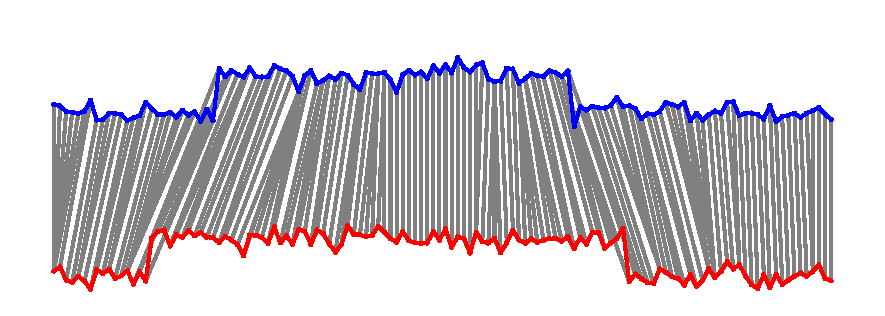
\includegraphics[width=.8\textwidth]{fig/dtw_warping_length}
         \caption{LDTW matches}
     \end{subfigure}
     \begin{subfigure}[b]{\textwidth}
          \centering
          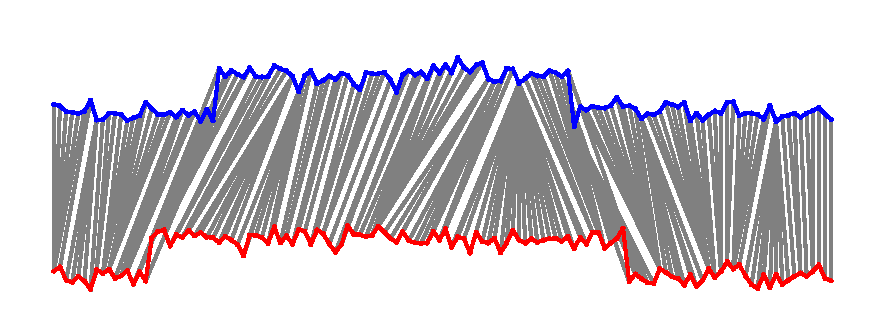
\includegraphics[width=.8\textwidth]{fig/dtw_warping_length_b}
          \caption{DTW matches}
      \end{subfigure}
    \caption{Compared matches obtained with DTW and its
    warping-length-constrained variant LDTW. Note the comparatively smaller
    temporal distrortions induced by LDTW.}
    \label{fig:ldtw}
\end{figure}

Moreover, our experiments on UCR Time Series Datasets~\cite{ucr} show that
this similarity measure, when used in a 1-Nearest Neighbor Classifier, leads to
a higher accuracy than other constrained DTW variants
(Sakoe-Chiba band and Itakura parallelogram).
